\section{Reachability Analysis on Hybrid Systems}

\subsection{Hybrid Automata}

Hybrid systems are a class of dynamical systems exhibiting both continuous flow and discrete jumps. They are usually systems composed of a discrete controller interacting with a physical environment. A popular class of formal models for hybrid systems are called \emph{hybrid automata}~\cite{}, whose definition is given as follows.

\begin{defn}
 A \emph{hybrid automaton} is defined by a tuple $\mathcal{A} = \tupleof{\loc, \var, \flow, \trans, \inv, \init}$ such that
 \begin{itemize}[-]
  \item $\loc$ is a finite set which consists of all discrete locations (or modes) of the system,
  
  \item $\var$ is a finite set which contains all continuous variables of the system,
  
  \item $\flow$ is a function associating each location a continuous dynamics which is defined by an ODE,
  
  \item $\trans$ consists of finitely many discrete jumps among the locations. A jump from $\ell$ to $\ell'$ is defined by a tuple $\tupleof{\ell, G, R, \ell'}$ such that $G\subseteq \reals^{|\var|}$, $R: \reals^{|\var|}\rightarrow \reals^{|\var|}$ are called the \emph{guard} and \emph{reset} respectively. The jump is enabled, i.e., allowed to take place, only if the guard $G$ is satisfied by the variable values. After the jump is made, the variable values are reassigned according to the reset $R$.
  
  \item $\inv$ is a function that defines an \emph{invariant}, i.e., a valid variable value range, $\inv(\ell) \subseteq \reals^{|\var|}$ for each location $\ell \in \loc$,
  
  \item $\init$ is a set which contains all initial states of the system.
 \end{itemize}
\end{defn}

\begin{example}
 We consider the motion of a bouncing ball. We introduce the variable $x$ to denote the height of the ball and $v$ to denote its velocity. Initially, the ball is static and is at the position that is $5$m from the ground. Then it falls down due to gravity. When the ball hits the ground while falling, then it is bounced up, that is, the velocity is reversed immediately with some loss in the speed. Therefore, we need one location whose state space is at most a 2-dimensional Euclidean space. Since the height $x$ should always be non-negative, the invariant of the location is $\{(x',v')\,|\,x' \geq 0\}$. The continuous motion of the ball can be described by the ODE $\dot{x} = v$, $\dot{v} = -g$ wherein $g$ is the gravitational acceleration. The bouncing action can be modeled by a self-loop jump whose guard is $\{(x',v')\,|\,x' = 0 \wedge v' < 0\}$ and reset is $x' := x$, $v' = 0.8v$. Figure~\ref{fig:bouncing_ball} shows the hybrid automaton. In the rest of the paper, we omit the identity mapping(s) in a jump reset.
\end{example}

\begin{minipage}{0.48\textwidth}
 \centering
 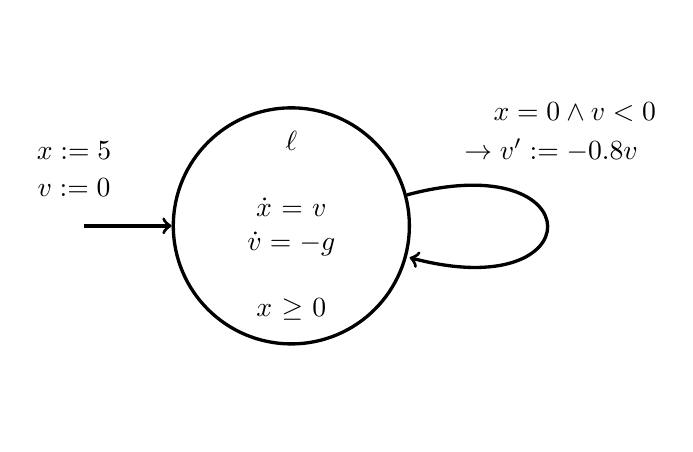
\begin{tikzpicture}[scale=1.2]
  \node[very thick, circle, text width=1.2cm, text centered, draw] (l) at (0,0) {$\ell$\\ \ \\ $\dot{x} = v$\\ $\dot{v} = -g$\\ \ \\ $x \geq 0$};
  \path[very thick, ->] (l) edge[loop right] (l);
  \node at (3,1.2) {$x = 0 \wedge v < 0$};
  \node at (2.75,0.8) {$\rightarrow v' := -0.8 v$};
  \node (dummy) at (-2.3,0) {};
  \path[very thick, ->] (dummy) edge (l);
  \node at (-2.3,0.8) {$x := 5$};
  \node at (-2.3,0.4) {$v := 0$};
  \node at (0,2) {};
  \node at (0,-2) {};
 \end{tikzpicture}
 \captionof{figure}{Hybrid automaton for a bouncing ball}\label{fig:bouncing_ball}
\end{minipage}
\hspace{1ex}
\begin{minipage}{0.48\textwidth}
 \centering
 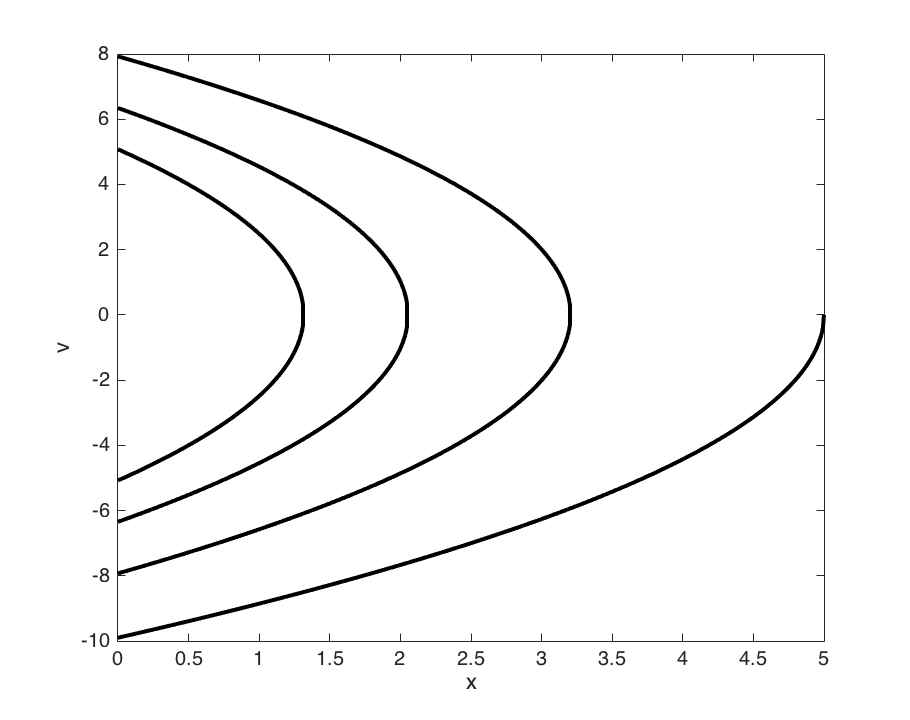
\includegraphics[height = 5cm]{images/bouncing_ball}
 \captionof{figure}{An execution of the hybrid automaton}\label{fig:execution}
\end{minipage}


A \emph{state} of a hybrid automaton $\mathcal{A}$ is denoted by a pair $(\ell, v)$ wherein $\ell$ is the current location and $v$ is a constant vector whose components denote the current values of the variables. A state $(\ell,v)$ can evolve to $(\ell', v')$ in the following two cases: (i) \emph{continuous evolution}, i.e., $\ell = \ell'$ and there is a solution $\varphi(t)$ of the ODE of $\ell$ such that $v = \varphi(t_1)$, $v' = \varphi(t_2)$, $t_1 \leq t_2$ and $\varphi(t) \in \inv(\ell)$ for all $t \in [0,t_2]$; (ii) \emph{discrete evolution}, i.e., there is a jump $\tupleof{\ell, G, R, \ell'}$ such that $v\in G$ and $v$ is updated to $v'$ according to $R$.

An \emph{execution} of a hybrid automaton is a sequence of states such that there is an evolution for each successive pair. As an example, Figure~\ref{fig:execution} shows an execution of the bouncing ball hybrid automaton over the time $[0,5]$.




\subsection{Reachability Analysis}







